\documentclass[12pt]{article}					% Začátek dokumentu
\usepackage{../../MFFStyle}					    % Import stylu



\begin{document}
Máme systém $x' = y, y' = u$, kde $|u| ≤ 1$.

\begin{priklad}[I]
	Pro bod $(x_0, y_0)$ ukažte, jak jej můžeme přivést do počátku.

	\begin{reseni}
		Jednoduchý způsob jak přivést systém do počátku je podívat se, co se stane, když zvolíme konstantní $u(t) = 1$ respektive $u(t) = -1$. V takovém případě se pohybujeme po parabolách $c + \frac{y^2}{2} = x$ ve směru rostoucího $y$ respektive po $c - \frac{y^2}{2} = x$ ve směru klesajícího $y$. Tedy pokud se dostaneme na správnou „polovinu“ $\frac{y^2}{2} = x$ nebo $-\frac{y^2}{2} = x$, tak už se dostaneme do počátku.

		Pokud je tedy $y_0 < (-\sign x_0) \sqrt{2|x_0|}$, tudíž jsme pod křivkou (sjednocení příslušných „polovin“ parabol), ze které se už umíme dostat do počátku, tak se můžeme po příslušné (té procházející $(x_0, y_0)$) $c + \frac{y^2}{2} = x$ dostat na tuto křivku. V opačném případě můžeme naopak využít trajektorií $c - \frac{y^2}{2} = x$, kde $y$ klesá, kterými se právě zase dostaneme do bodů, ze kterých už můžeme jít do počátku.

		\begin{center}
			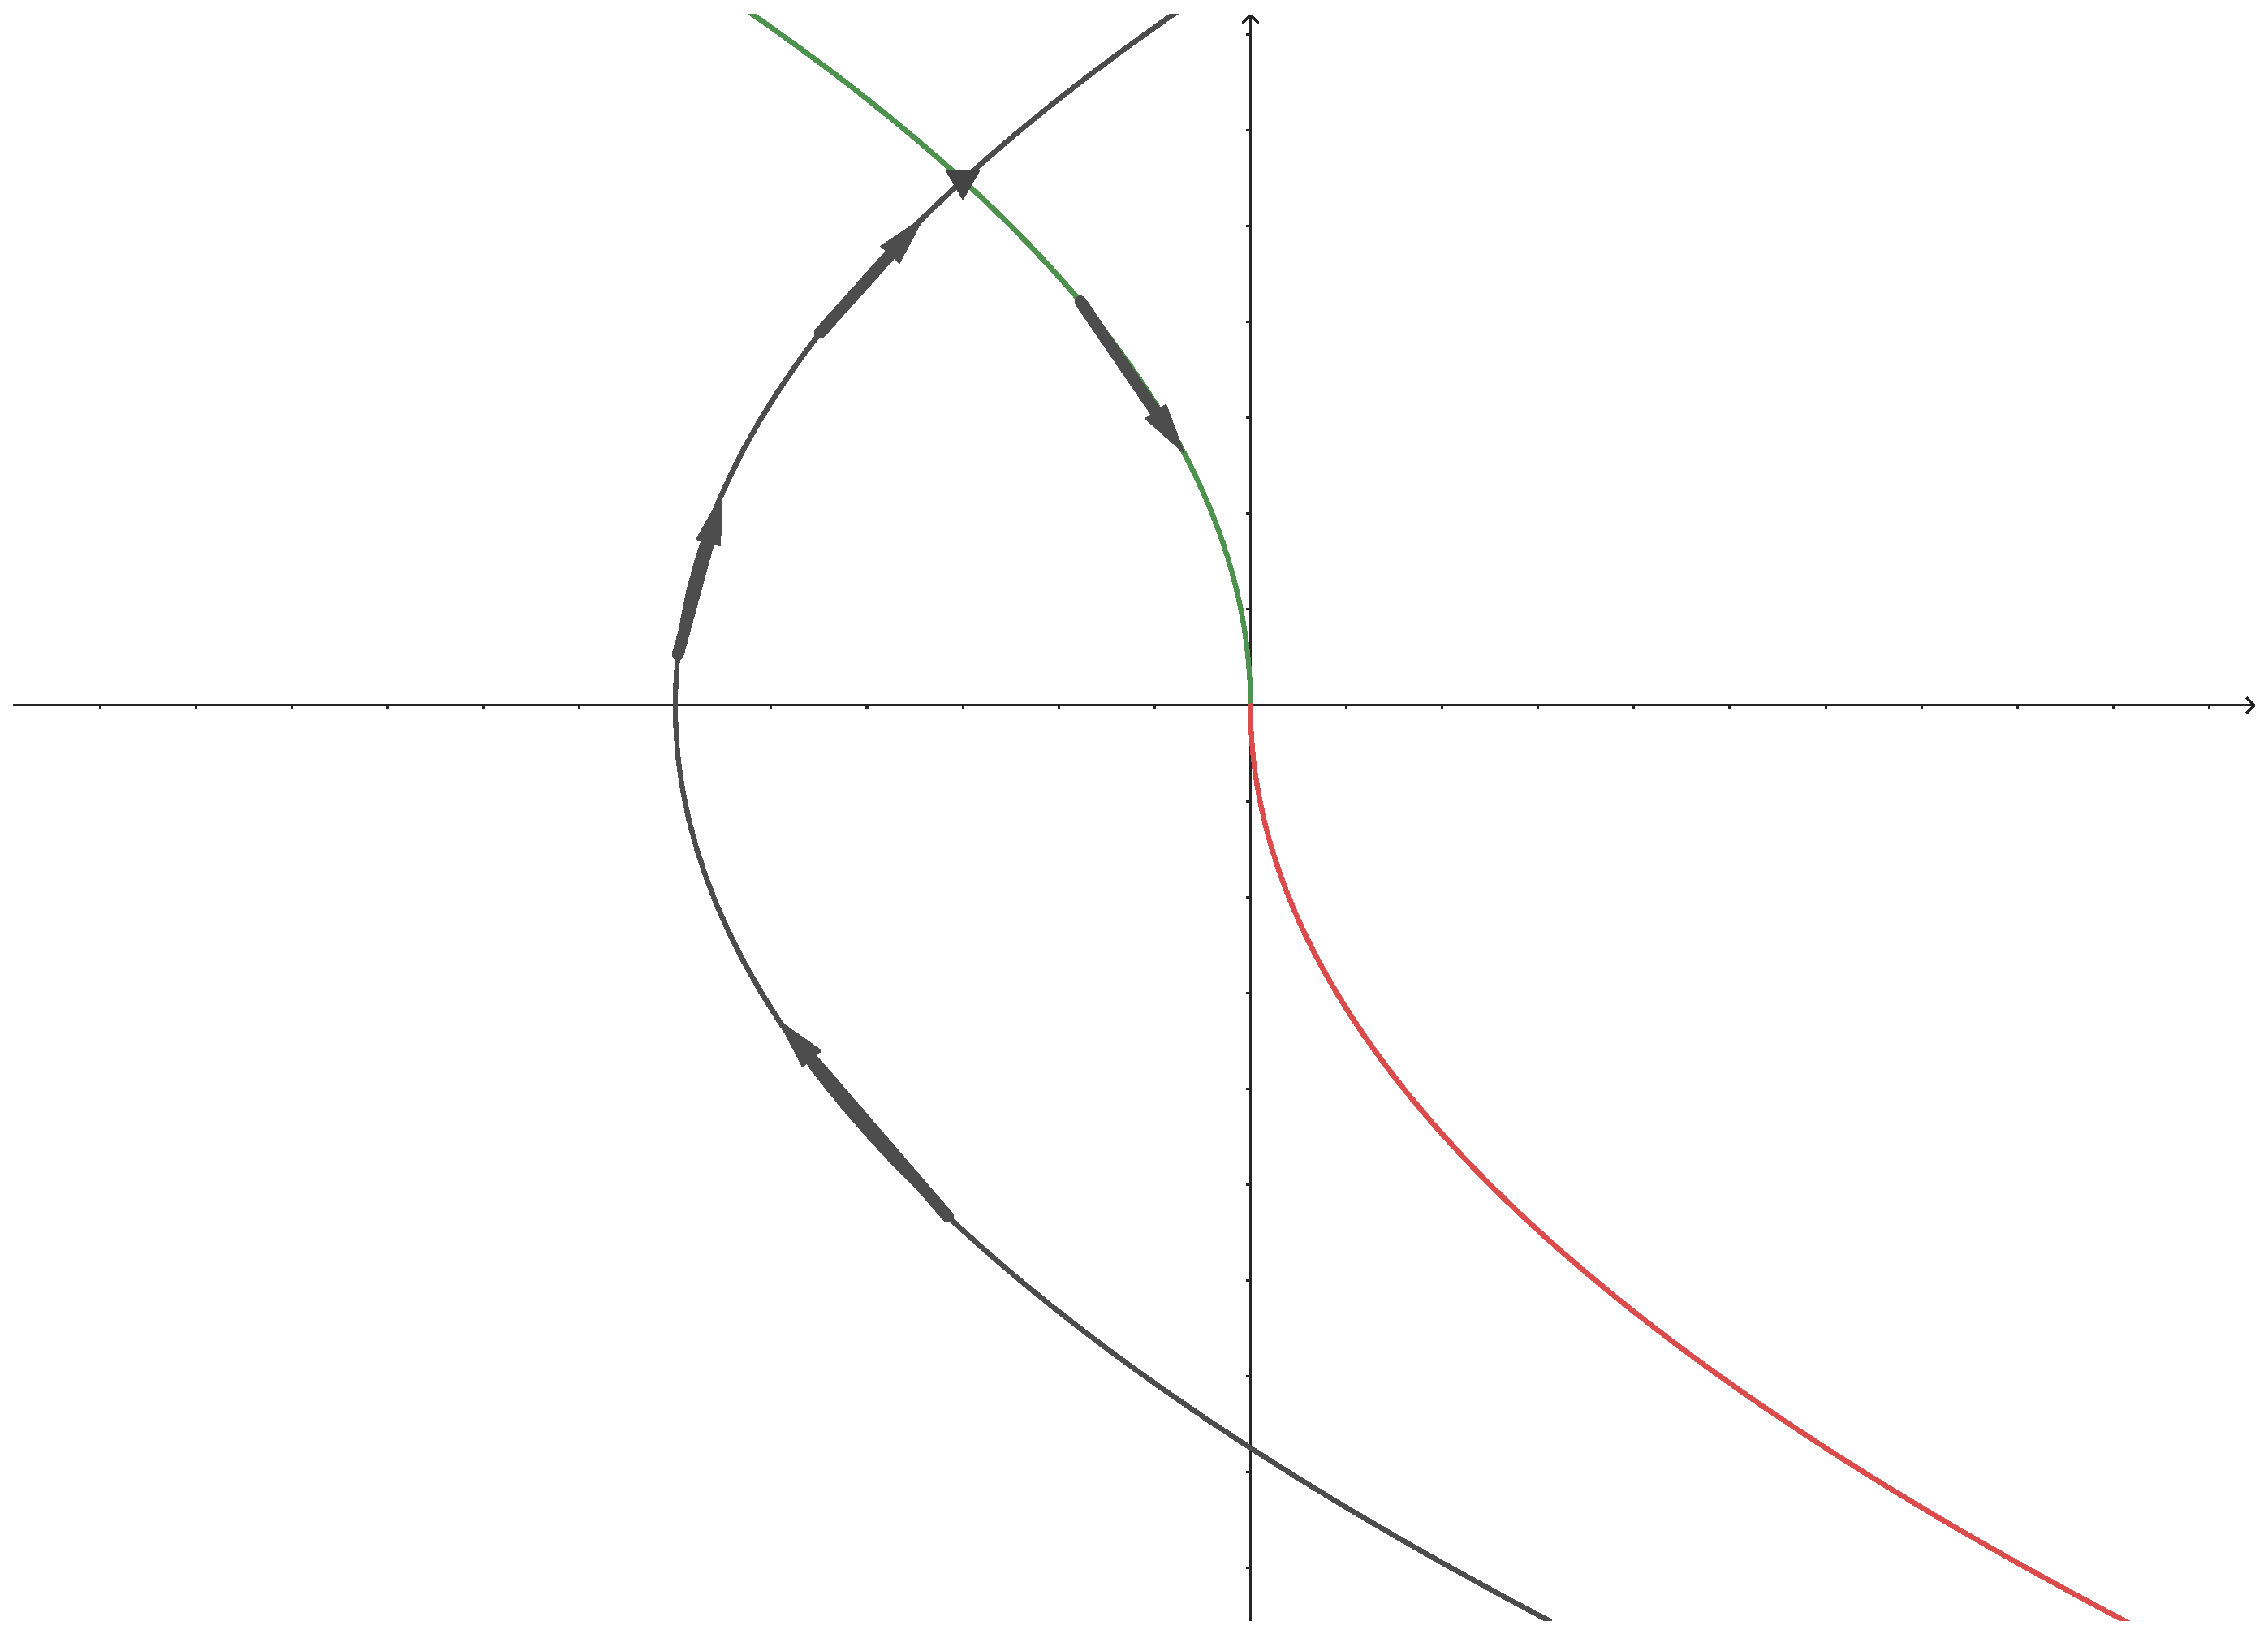
\includegraphics[width=0.5\textwidth]{ODR2_DU1.eps}
		\end{center}

		(V $(0, 0)$ následně můžeme zůstat nastavením $u(t) = 0$.)
	\end{reseni}

	\pagebreak

	Ze všech příslušných trajektorií ukažte, že minimální čas nastává pro funkci $u(t)$ nabývající pouze hodnot $1$, $-1$.

	\begin{dukazin}
		%Pokud jsme na křivce $y = (-\sign x) \sqrt{2|x|}$, tak se můžeme dívat, jak se nejrychleji dostat na $x = 0$. Víme, že
		%A obdobně pro dolní omezení. Tedy nejrychleji se do $x = 0$ dostaneme tak, že $u(t) = ±1$, a díky tomu, jak jsme si řešenou křivku definovali, tak při dosažení $x = 0$ budeme v počátku.
		%
		%$$ x(t) = \int_{t_0}^t y(s) ds + x_0 = \int_{t_0}^t y_0 + \int_{t_0}^s u(s_2) ds_2 ds + x_0 ≤ x_0 + y_0·t + \frac{(\sup_{[t_0, t]} u)^2}{2}. $$
		%Pokud jsme pod touto křivkou pro $x < 0$ (nebo nad ní pro $x > 0$), tak se stejným způsobem chceme dostat do do $x = 0$, takže nastavíme $u(t) = ±1$ ($+$ nebo $-$ podle toho, zda $x < 0$ nebo $x > 0$), načež se někdy dostaneme na inkriminovanou křivku a tu už jsme vyřešili.
		Nemá smysl mít $y = 0$ po delší časový interval než samotný bod. Tím pádem nás $u$ zajímá pouze v bodech, kde $y ≠ 0$, neboť při změnění $u$ v množině míry nula (jednotlivých bodech, jelikož je $y$ spojitá, tak takových osamělých bodů nemůže mít více než spočetno) se nám řešení nezmění (pokud nepřestane existovat).

		Mějme tedy bod, kde BÚNO $y_0 = y(t_0) > 0$ (případ $y_0 < 0$ je analogický). Jelikož je $y$ spojitá, máme nějaké okolí $[t_1, t_2]$ času $t_0$, že $\forall t \in [t_1, t_2]: y(t) > 0$. Zajímá nás, jak se můžeme dostat nejrychleji z $(x_1, y_1) = (x(t_1), y(t_1))$ do $(x_2, y_2) = (x(t_2), y(t_2))$.

		Speciálně se podíváme na vývoj $x$ – jelikož $y > 0$, tak $x$ roste. Abychom se dostali nejrychleji z $x_1$ do $x_2$, tak $x' = y$ musí být co největší. To bude, když na začátku bude $y'(t) = u(t) = 1$, neboť $y = \int_{t_1}^t u(s) ds + y_0 ≤ (t - t_1)·\sup{u(s)} + y_0 ≤ (t - t_1) + y_0$, kde rovnost nastává právě, když $u = 1$ skoro všude (tj. můžeme předpokládat všude). Když se na situaci podíváme s časem „jdoucím pozpátku“, stejným argumentem dokážeme, že na konci musí být $u = -1$, tedy budeme mít pořád $u = 1$ a pak $u = -1$.

		Takže každé řešení můžeme v okolí každého bodu $y ≠ 0$ nezhoršit tím, že použijeme $u = ±1$. Konkrétně pokud je na nějakém intervalu $u ≠ ±1$, tak dostáváme výše ostrou nerovnost, takže můžeme řešení dokonce zlepšit.
	\end{dukazin}

	Je nejrychlejší trajektorie zároveň nejkratší trajektorie?

	\begin{reseni}
		Není, neboť například z bodu $(-1, 0)$ se do bodu $(0, 0)$ můžeme dostat tak, že chvíli budeme mít $u(t) ≥ 0$, než se dostaneme do $y = \epsilon$. Pak budeme mít $u(t) = 0$ po nějakou dobu, čímž zvětšíme $x$ až skoro k nule, načež zvolíme $u(t) ≤ 0$, abychom se dostali do $(0, 0)$.

		Takto jsme se pohybovali téměř po úsečce, takže zřejmě „nejkratší trajektorií“ (přímo po úsečce se pohybovat nemůžeme), ale očividně bude o dost pomalejší (má velmi malou derivaci v $x$) než po parabolách.
	\end{reseni}
\end{priklad}

\pagebreak

Definujme přímku procházející body $(x_1, y_1)$ a $(x_2, y_2)$ jako trajektorii, která nás přivede z bodu $(x_1, y_1)$ do bodu $(x_2, y_2)$ za nejkratší čas.

\begin{priklad}[II]
	Jak vypadají přímky procházející počátkem?

	\begin{reseni}
		Do počátku musí přijít po už zmiňované křivce, tj. po některé z daných dvou parabol (protože musí být $u = ±1$). Zároveň pokud z počátku ještě někam pokračuje, tak po druhé „polovině“ dané paraboly, neboť z „poloviny“ jedné paraboly se umíme dostat do „poloviny“ druhé paraboly rychleji (v počátku máme zbytečně $x' = 0$), takže by to nesplňovalo definici přímky. Tedy jedněmi přímkami jsou celé paraboly $±\frac{y^2}{2} = x$.

		Nebo může do přímky patřit parabola až do té doby než protíná inkriminovanou křivku, načež se pokračuje po této křivce do počátku (pak ale pokračovat nemůže, protože z bodů mimo inkriminovanou přímku se dá dostat na druhou „polovinu“ dané paraboly rychleji než po inkriminované křivce).

		Nebo může v počátku přímka začínat, pokračovat po „polovině“ jedné z parabol procházejících počátkem a v nějakém bodě pokračovat po parabole procházející tímto bodem. Ale zase nemůže obsahovat nic jiného, nebo se „lámat“ v dalším bodě.

		\begin{center}
			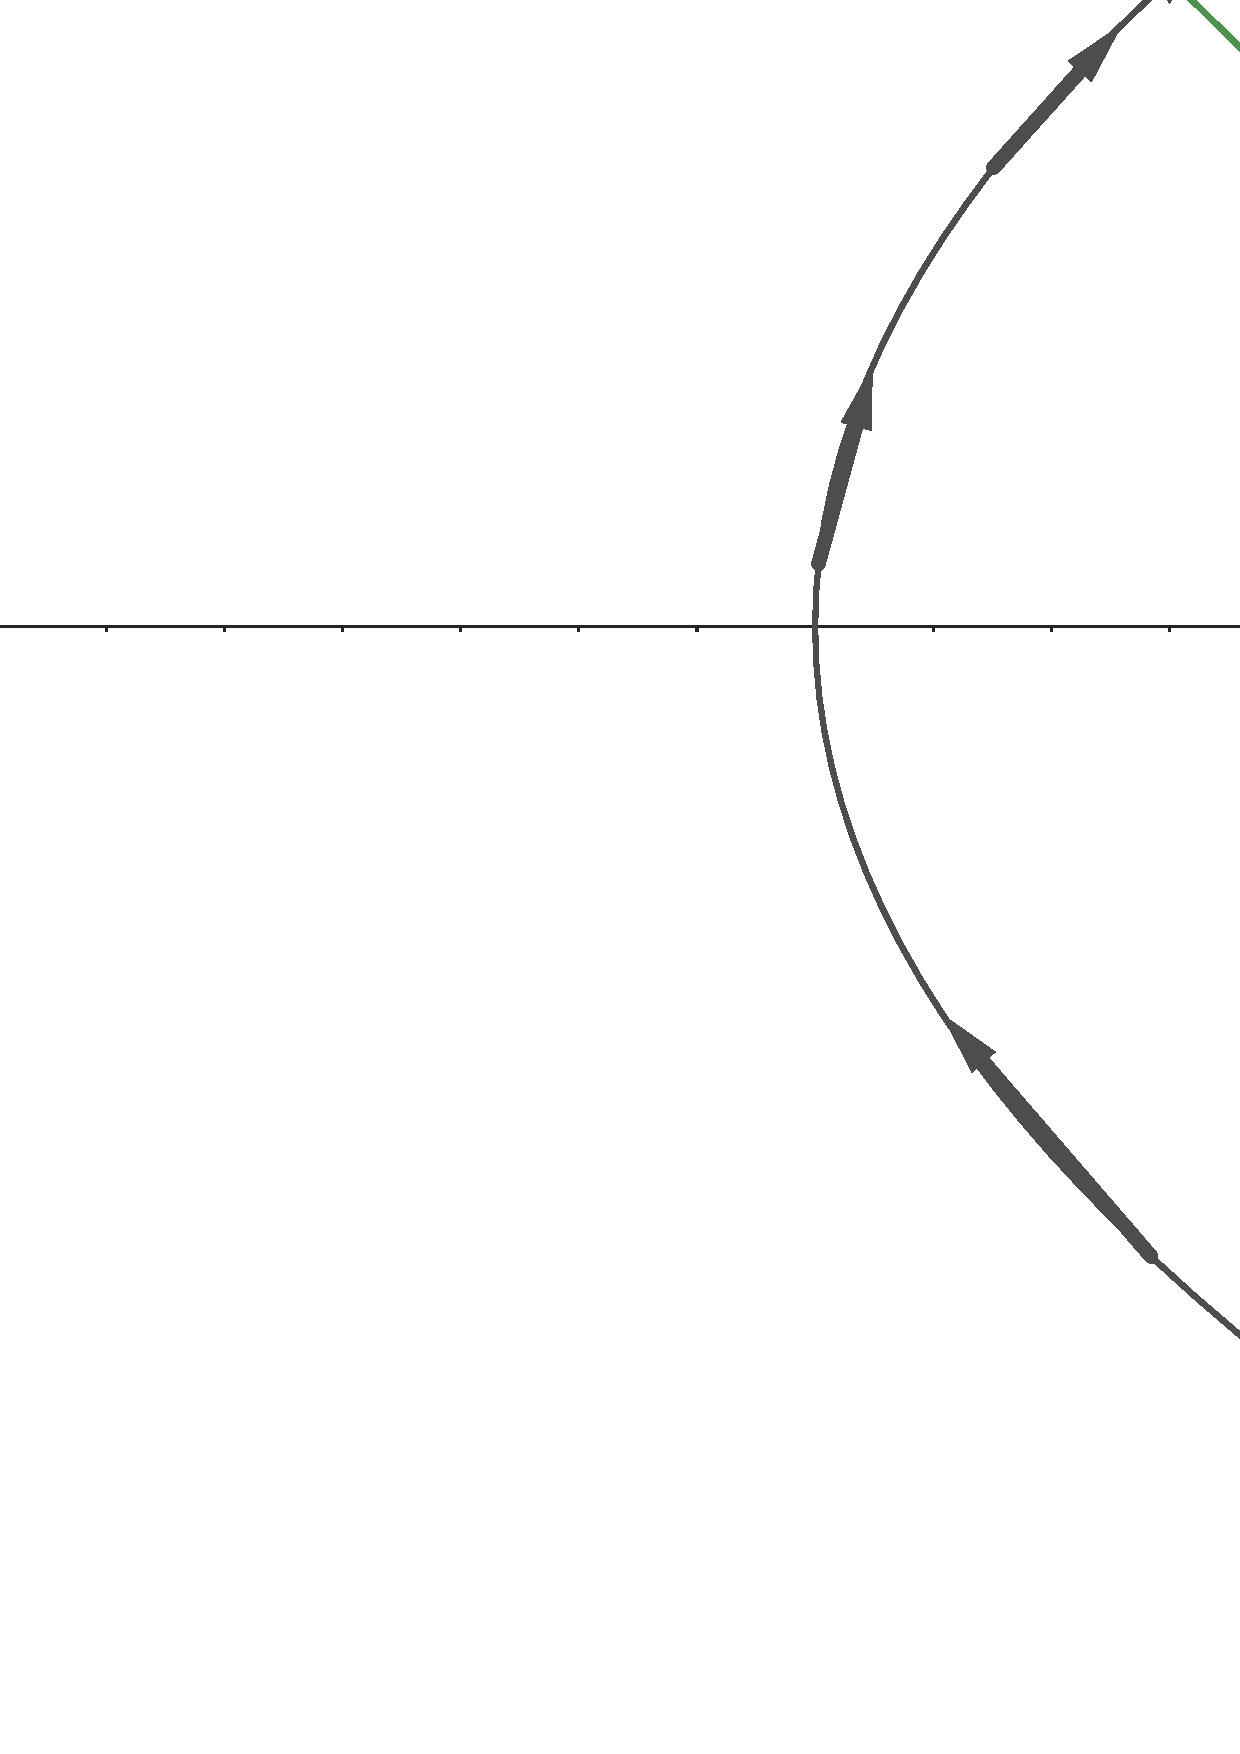
\includegraphics[width=0.5\textwidth]{ODR2_DU1.png}
		\end{center}
	\end{reseni}
\end{priklad}

\begin{priklad}[III]
	Jak vypadají obecné přímky (nemusí tedy nutně procházet počátkem)?

	\begin{reseni}
		Vypadají úplně stejně, jen dvě hlavní paraboly budou mít vrchol v jiném bodě na ose $x$, jelikož musí být zase (alespoň v malém okolí nějakého bodu) paraboly a „lámat“ se mohou nanejvýš jednou.
	\end{reseni}
\end{priklad}

\end{document}
